\documentclass[11pt]{report}

\special{papersize=8.5in,11in}

\topmargin -0.5in \oddsidemargin 0.00in \evensidemargin 0.00in
\textwidth 6.75in \textheight 9.0in \headheight 0.25in \headsep
0.25in \footskip 0.5in \hoffset 0in \marginparpush 0.0in
\marginparwidth 0.0in \marginparsep 0.2in

\setcounter{page}{1}

\newcommand{\D}{\displaystyle}\newcommand{\T}{\textstyle}
\newcommand{\e}{{\mathrm{exp}}}
\newcommand{\dd}{{\mathrm d}}
\newcommand{\comment}[1]{}
\newcommand{\mb}{\mathbf}
\reversemarginpar

\usepackage[final]{graphicx}
\usepackage{fancyhdr}
%\graphicspath{{Papers/}}
\usepackage{amsthm,amssymb,amsmath}
\usepackage{cite}
\usepackage{geometry}
\usepackage{amsmath}
\usepackage{booktabs}
\usepackage{color}
\usepackage{setspace}
\usepackage{subfigure}
\usepackage{url}
%\usepackage{algorithm}
\usepackage{algorithmic}
\usepackage[ruled]{algorithm2e}
%\usepackage[top=2.5cm, bottom=2.5cm, right=3.5cm, left=3.5cm]{geometry}
\geometry{a4paper,scale=0.8}
\setcounter{secnumdepth}{3}

\title{Research Progress Report}

\author{Botao Zhu}

\begin{document}
	
	\maketitle
	\lhead{\sf Research Progress Report-9th} \chead{} \rhead{\sf Botao Zhu}
	\lfoot{CTRG, University of Saskatchewan} \cfoot{} \rfoot{Page \thepage}
	\renewcommand{\footrulewidth}{1.0pt}
	\renewcommand{\headrulewidth}{2.0pt}
	\renewcommand{\arraystretch}{1.3}
	\pagestyle{fancy}
	
	\renewcommand{\thesection}{\arabic{section}}
	
	\section{Reading and Research Activities}
 
	


	\textbf{Considering energy efficient and density clustering protocol based on kernel soft k-Means for wireless sensor network}
	
	%%%%
	% there are a few research on Leach for non-uniform area. the most of modified leach protocol focus on savig energy and extedning the lifetime of wsn. mainly on following aspects: 1. improving the selection of ch, like considering residual energy  2.improving clustering methods, like kmeans. in detail, comparing kmeans with other algorithms, the initial centroid, . 3.choosing two or more chs in the cluster. 4. controlling normal nodes to send data.
    
	
	\subsection{Problem statement}
	At present, most of the research on wireless sensor networks are based on the assumption that the nodes are evenly distributed. Different application scenarios may result in non-uniform distribution of nodes. \cite{5693275} \cite{doi:10.1155/2013/289527} proposed W-LEACH algorithm to handle non-uniform network, which chooses a number of sensors in each cluster to send data to their CHs based on a fixed percentage. The target is to reduce the number of sending sensors for extending the lifetime of network. However, it may result in the loss of important information. Hence, it is significant to study non-uniform distributed wireless networks. The research can be divided into two aspects: clustering algorithm and cluster head selection.\\
	
	\noindent K-means clustering algorithm is used by \cite{6375088} firstly in LEACH of wireless sensor networks. However, there are some drawbacks. Firstly, K-Means algorithm chooses the initial centroid randomly, which cannot ensure that clustering is optimal. If the initial centroid is far away from the cluster's true centroid, it will cause the result that the number of iterations required to optimize the centroid takes longer and an incorrect clustering may be obtained. \\
	
	\noindent Secondly, the node with the highest residual energy in the cluster is elected as the cluster head(CH). It can lead to a potential problem:unbalanced energy load and excessive energy expenditure. For example, node A in Fig.\ref {cha} has higher residual energy than other nodes in the cluster, which means node A can be elected as the CH with the highest probability. However, this way enables the other nodes in the same cluster to send data in the opposite direction to the base station, causing higher energy consumption. 
	\begin{figure}[!h]
		\centering
		\includegraphics[width=0.6\linewidth]{cha.jpg}
		\caption{A example of CH selection}
		\label{cha}
	\end{figure}
	
	\noindent Thirdly, it does not consider that some of sensor nodes in a cluster can be reallocated to another cluster. As shown in Fig.\ref{cha1}, if we use hard classification algorithm, K-Means, node $n$ belongs to cluster B. However, if we consider this question from the perspective of probability, node $n$ joins the cluster B with a certain probability, $55\%$. Then, it will have a $45\%$ probability to join the cluster A. Because the density of cluster B is greater than that of cluster A, node $n$ can be allocated to cluster A in order to reduce the stress of CH of cluster B. 
	
	\noindent Fourthly, because each cluster only selects one cluster head, cluster head's energy will be depleted quickly for aggregating, compressing and transmitting information when there are too many sensor nodes in the cluster. \cite{Sangameswaran} proposed a method to prolong the lifetime of each round by balancing the energy consumption of the nodes. The nodes are divided into three types in each cluster: CH, vice CH and member nodes. The vice CH plays the role of CH when the CH dies before the completion of current round, which can diminish the frequency of re-clustering and extend network lifetime. \cite{doi:10.1155/2016/5040475} also comes up with a similar concept. After stable clusters have been achieved, CH node assigns its two nearest nodes as CHs, which can ensure load balancing. However, neither of them considers the problem of cluster size, that is non-uniform distributed wireless networks. In Fig.\ref{cha1}, when CHs of cluster B runs out of energy, CHs of cluster A still have a lot of energy because it contains fewer member nodes, which can result in unbalanced load.\\
	
	\begin{figure}[!h]
		\centering
		\includegraphics[width=0.6\linewidth]{cha1.jpg}
		\caption{A example of non-uniform wireless network}
		\label{cha1}
	\end{figure}
    
    \noindent As mentioned above, our goal is to improve these four problems. 1) optimizing the selection of the initial centroid of clustering algorithm by using kernel density estimation. 2) adjusting cluster size dynamically to balance node load by soft K-Means. 3) determining the location of CHs according to the energy density by kernel density estimation. 4) selecting the number of CH according to the size of clusters.
    
    
	
	
	\subsection{Soft K-Means}
	\cite{report} K-Means is the simplest clustering algorithm in unsupervised learning, which partitions the data set in to $k$ clusters using some distance measurement methods, like Euclidean distance. It is a hard clustering method, that is to say the membership degree of one node has only two values 0 and 1 for a specific class. However, in some cases, there are a few data points for which it is not quite so obvious to which cluster they belong. Soft K-Means clustering decides to which degree each data point belongs to , the assignments to clusters will be probabilistic. Generally speaking, soft K-Means clustering can be seen as the problem of finding $k$ cluster centroids with the aim of minimizing the error function. Given a set of data points $X = \{x_1,x_2,...,x_n\}$, the error function is
	
	\begin{equation}
	E\left(\mu_1,\mu_2,...,\mu_k\right) = \sum_{i=1}^{k}E\left(\mu_i\right) = \sum_{i=1}^{k}\sum_{j=1}^{n}z_{ij} ||x_j-\mu_i||^2
	\end{equation}
	where $\mu_i$ is the centroid of each cluster, $z_{ij}$ is the indicator variable. \\ 
	For the traditional K-Means clustering 
	\begin{equation}
	z_{ij} = \left\{ \begin{array}{ll}
	1, \text{if}\,x_{j} \in C_{i}\\
	0, \text{otherwise}
	\end{array} \right.
	\end{equation}
	where $C_{i}$ represents cluster $i$, this equation means whether $x_{i}$ belongs to cluster $C_{i}$. However, $z_{ij}$ is not a integer value for soft K-Means clustering 
	\begin{equation}
	\label{eq1}
	z_{ij} = \frac{e^{-\beta ||x_{j}-\mu_i||^2}}{\sum_{l=1}^{k}e^{-\beta||x_{j}-\mu_l||^2}}
	\end{equation}
	where $\beta$ is the stiffness parameter and greater than 0. 
	From equation (\ref{eq1}), we can get $z_{ij} \in [0,1]$ and $\sum_{i}z_{ij}=1$.\\
	How to update the centroid $\mu_{i}$ of each cluster until convergence? For a specific class $C_{i}$
	\begin{equation}
	\label{eq2}
	E\left(\mu_{i}\right) = \sum_{j=1}^{n}z_{ij}||x_{j}-\mu_{i}||^2
	\end{equation}
	the target is to minimize the error function, so the problem can be turned into the following optimization problem
	\begin{equation}
	e = \text{argmin}\sum_{j=1}^{n}z_{ij}||x_{j}-\mu_{i}||^2
	\end{equation}
	which is a convex function and has a unique minimum value. The equation (\ref{eq2}) can be written as
	\begin{eqnarray}
	E\left(\mu_{i}\right) &=& \sum_{j=1}^{n}z_{ij}\left(x_j-\mu_{i}\right)\top \left(x_j-\mu_{i}\right)\\
	 &=& \sum_{j=1}^{n}z_{ij}\left(x_j \top x_j-2x_j \top \mu_{i} + \mu_{i} \top \mu_{i}\right)
	\end{eqnarray}
	deriving $E\left(\mu_{i}\right)$ with respect to $\mu_{i}$ and denoting to zero, we can have
	\begin{equation}
	\label{eq3}
	\mu_{i} = \frac{\sum_{j=1}^{n}z_{ij}x_j}{\sum_{j=1}^{n}z_{ij}}
	\end{equation}
	Each cluster updates the centroid according to equation (\ref{eq1}) and (\ref{eq3}) until the probabilities of the clusters in which the data points are located remain unchanged or the maximum number of iterations are reached. \\

	%\noindent The advantage of applying soft K-Means clustering in wireless sensor network is each sensor node joins the clusters with a certain probability, which can prevent some clusters from having too many nodes. Assuming two adjacent cluster A and B, the number of nodes in cluster A is greater than that in cluster B, shown in Fig.\ref{fig1}. It will lead to a serious case that the cluster head node of cluster A consumes energy quickly because cluster head node will take more energy to deal with the message from member nodes within its cluster. In this case, some nodes at the intersection edge of cluster A and B will join cluster B with greater probability to reduce the stress of cluster head node of cluster A in order to avoid energy hole. However, the random selection of initial clustering centroid makes the clustering results fall into local optimum, and the accuracy of soft K-Means algorithm is low because of the noise points and the uncertain clustering. 
	
	\subsection{Kernel density estimation}
	The first law of geography states that all things are interrelated. The closer they are, the stronger they are. Kernel density estimation is based on this law, its value decreases gradually with the increase of the central radiation distance. From two-dimensional or three-dimensional surface of density, we can intuitively acquire the features of point sets. 
	
	\noindent \cite{reportkernel} \cite{doi:10.1080/02331880500439782}Kernel density is one of the non-parametric estimation methods used to estimate the unknown density function. Each point is covered with a smooth surface. The surface value at the location of the point is the highest and decreases with the increase of distance until the value is zero when the distance equals the search radius, which looks like the density map of Gauss distribution function. Then, the values of kernel density estimation of all points are superimposed and a set of points is transformed into a surface showing continuous density changes. 
	
	\noindent Supposing $X=\{x_1,x_2,\dots,x_n\}$ is independent distributed random variable, density function is $f(x)$, $x\in R$
	\begin{equation}
	\hat{f}(x) = \frac{1}{nh} \sum_{i=1}^{n}K\left(\frac{x-x_i}{h}\right)
	\end{equation}
	where $\hat{f}(x)$ is the kernel density estimation of $f(x)$,  $K$ is the kernel function, $h$ is the bandwidth, $n$ is the number of points in the bandwidth range. \\
	
	\noindent Kernel function is usually required to satisfy the following conditions:
	\begin{equation}
	K\left(-\mu\right) = K\left(\mu\right)
	\end{equation}
	\begin{equation}
	\text{Sup}|K\left(\mu\right)| < \infty
	\end{equation}
	$\hat{f}(x)$ is related not only to the data, but also to the kernel function and the window width parameter $h$. Here are the usual kernel functions:\\
	\noindent (1) Gaussian kernel
	\begin{equation}
	K\left(\mu\right) = \frac{1}{\sqrt{2\pi}}e^{\frac{\mu^2}{2}}
	\end{equation}
	\noindent (2) Boxcar kernel
	\begin{equation}
	K\left(\mu\right) = \left\{ \begin{array}{ll}
	1, |\mu|\leq 0.5\\
	0, |\mu|> 0.5
	\end{array} \right. 
	\end{equation}
	\noindent (3) Epanechnikow kernel
	\begin{equation}
	K\left(\mu\right) = \left\{ \begin{array}{ll}
	\frac{3\left(1-u^2\right)}{4},|\mu| \leq 1\\
	0,|\mu|>1
	\end{array} \right.
	\end{equation}
	
	\noindent We generate three sets of random numbers by Gauss function and implement kernel density estimation for them. Fig.\ref{2d} and Fig.\ref{3d} show the density distribution graph of two-dimensional and three-dimensional respectively. The discrete point set is transformed into a smooth density map, which shows its spatial distribution. The higher the density value, the higher the aggregation degree of the point is.\\
	\begin{figure}[!h]
		\subfigure[original data]{
			\begin{minipage}[h]{0.5\linewidth}
				\centering
				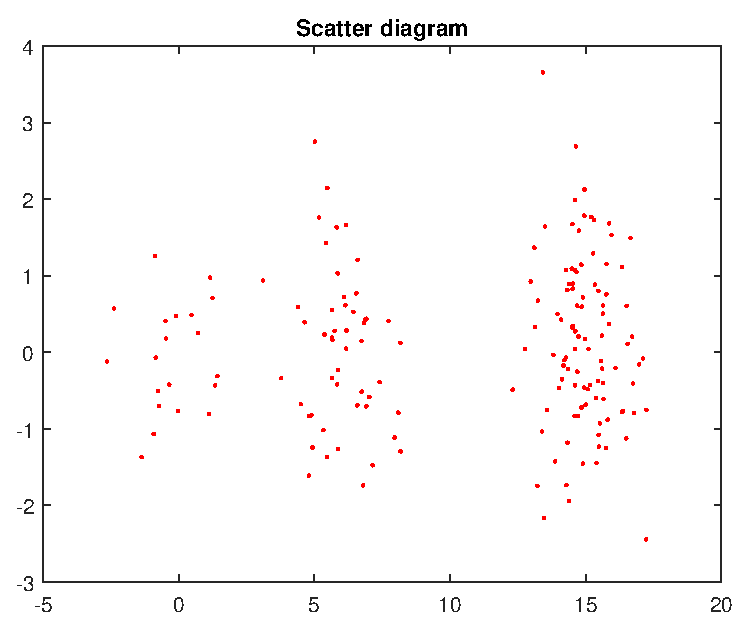
\includegraphics[width=3in]{original.eps}
				\label{original}
			\end{minipage}
		}
		\subfigure[2D]{
			\begin{minipage}[h]{0.5\linewidth}
				\centering
				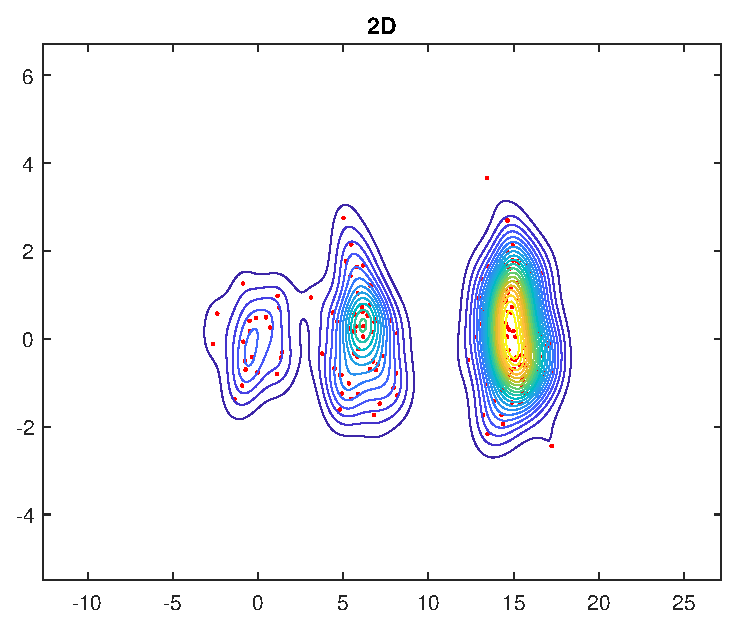
\includegraphics[width=2.5in]{2d.eps}
				\label{2d}
			\end{minipage}
		}
	    \subfigure[3D]{
	    	\begin{minipage}[h]{0.5\linewidth}
	    		\centering
	    		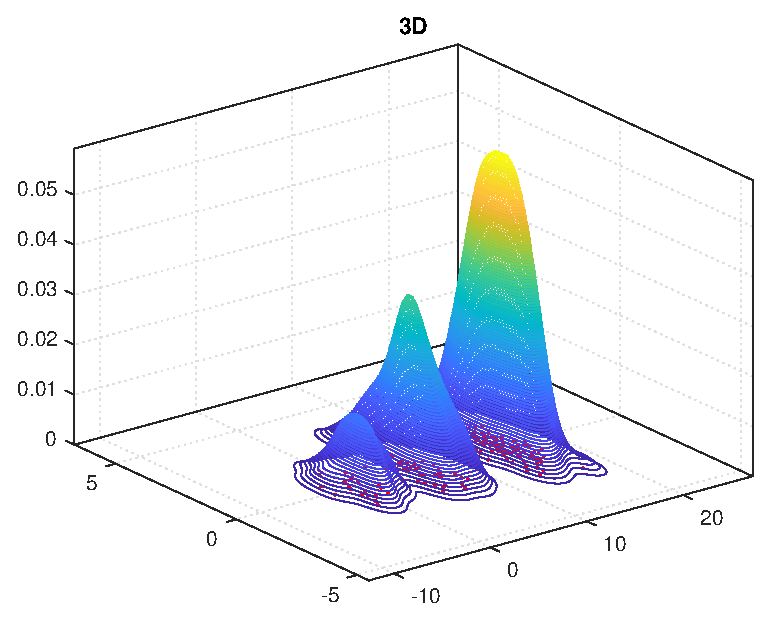
\includegraphics[width=2.5in]{3d.eps}
	    		\label{3d}
	    	\end{minipage}
	    }%
		\centering
		\caption{A example of kernel density estimation}
		\label{}
	\end{figure}
	%\noindent Firstly, the data samples are estimated by their position attributes to obtain a image which can show continuous density changes. The pixel value of the image represents the density of the location in the data samples. Setting a threshold, the image is divided into high-density areas and low-density areas. Then, the highest density points are extracted in some high density ares to form maximum density point set. Maximum density point set is used as clustering center, and the number of maximum density point set is used as K value. The maximum density points in a certain region are obtained, but the clustering effect is not good with the points in the low density region, so the maximum density point set is only obtained in the high density region.


	\subsection{Network Model and Energy Model}
	\subsubsection{Network Model}
	We have following assumptions regarding the network model \cite{article} \cite{7763028}:\\
	(a) The BS is a high energy node and is located far away from the extremities of the sensor network.\\
	(b) All sensor nodes having the same computational and transmission capabilities. In other words, all nodes are capable of acting as CH nodes.\\
	(c) The sensor nodes can vary the power with which they transmit signals according to the received signal strength indication of a particular node.\\
	(d) The sensor nodes scans its environment at a fixed rate and will contain data to be sent to the BS at all intervals.\\
	(e) The sensor nodes and BS are all static after deployment.\\
	(f) The sensor nodes in general have location information such as a GPS support.\\
	(g) The CHs perform data compression to reduce the amount of bits transmitted to the BS.\\
	(h) The BS indicates all nodes to reinitiate clustering when all the CH nodes in the network have insufficient energy.
	
	\subsubsection{Energy model}
	Because the main energy consumption of the protocol is only for receiving and sending data, the first order radio model as the energy model is in line with the needs \cite{1045297}.	As shown in Fig. \ref{fig3}, the energy consumption of nodes comes  from the sum of the energy consumption of signal transmitting, signal amplifying and receiving. 
	\begin{figure}[h!]
		\centering
		\includegraphics[width=0.6\linewidth]{firstordermodel.jpg}
		\caption{First order ratio model}
		\label{fig3}
	\end{figure}
    The longer transmission distance each node has, the more the signal intensity will lose. Assuming the transmission distance is $d$, whenever the data of K bit is transmitted or received, the energy consumption formula of the transmitting is as follows\\
	\begin{equation}
	E_{send} = E_{TX\_elec}(k) + E_{TX\_amp}(k,d) = k\times E_{static} + k\times \sigma\times d^\beta
	\end{equation}
	the energy consumption formula of the receiving
	\begin{equation}
	E_{receive} = E_{RX\_elec}(k) = k \times E_{static}
	\end{equation}
	$E_{static}$ is the energy consumption of receiving and transmitting. Amplification multiples of signal amplifier is expressed as $\sigma$, $\beta$ is the route loss index. We need to choose the corresponding energy consumption model according to the length of transmission path for calculating the energy of data transmission. In the first-order radio energy consumption model, there are two kinds of distance $d$: self-space model and multi-path fading model. Free space model will be used at close range, and multi-path fading model will be used at long range. 
	\begin{equation}
	\left\{ \begin{array}{ll}
	\sigma_{fs}\times k \times d^2 & d \leq d_0 \\
	\sigma_{amp} \times k \times d^4 & d > d_0 \\
	\end{array} \right.
	\end{equation}
	$\sigma_{fs}$ and $\sigma_{amp}$ represent the energy consumption parameters of amplifier of free space model and multi-path fading model respectively.

	
	
	\subsection{Proposed Algorithm}
	 The protocol is divided into many rounds. Each round contains setup phase and steady phase. In this research, we only focus on the setup phase and  improve some existing methods. During the setup phase,  the BS station gathers the location and residual energy of each node in the whole wireless network. Also, it generates k initial centers by kernel density estimation as the input of clustering algorithm, soft K-Means, which can avoid to get the results of local optimum by traditional K-Means clustering method. And then, classification algorithm is implemented. Each node calculates the distance between itself and center points and chooses to join the nearest cluster with a certain probability. At the same time, if the nodes on the edge of two clusters have similar distance to these two cluster centers, they will preferentially join the cluster with smaller density. After clustering, the final cluster centers are selected according to the energy density by kernel density estimation. The detailed discussion is given below.
	
	\subsubsection{Selection of Initial Cluster Heads}
	 Kernel density estimation is used to assign the initial center of the soft K-Means. Since the soft K-Means randomly choose the initial centroid, it is not guaranteed that clustering by the soft K-Means is optimal. The algorithm is described below.\\
	 \textbf{Step 1:} Kernel density estimation is applied to sample data to obtain a image with continuous density.\\
	 \textbf{Step 2:} The image is divided into low density area and high density area.\\
	 \textbf{Step 3:} Focus statistical tool is used to obtain max density point sets.\\
	 
	 \begin{algorithm}[H]
	 	\caption{Selection of initial cluster heads}
	 	\label{alg1} 
	 	\LinesNumbered %show number
	 	\KwIn{A set of $n$ data items $X = \{x_1,x_2,\dots,x_n\}$}
	 	\KwOut{Max density point sets}
	 	Kernel density estimation for $X$\;
	 	Selecting high density and low density areas\;
	 	Obtaining max density point sets as the input of clustering algorithm
	 \end{algorithm}
	
	
	\subsubsection{Cluster Formation}
	 Compared with the K-Means algorithm, our proposed algorithm will take one more step after the classification convergence, assigning nodes at the edge of the clusters to join the approximate cluster. We discuss this problem in two scenarios.\\
	 \textbf{Scenario 1:} The node N is at the edge of two clusters, shown in Fig. \ref{fig5}. The distance from node N to the center of cluster B is a little bigger than that from node N to the center of cluster A, which means it has a higher probability to join cluster A. However, if we consider the density of cluster, it is a different story. Cluster A has 5 member nodes and cluster B has 10 member nodes. Assuming that the time interval for each node sending messages to CH are consistent, CH of cluster B will deal with more information from member nodes. So, the better way is that the node N chooses to join cluster A, which can reduce the energy consumption of CH of cluster B and balance energy load. We define that when the difference between the probability of node N joining two different clusters is less than 10$\%$, node N will join the cluster with low density. Otherwise, it will join the cluster with high probability.\\
	 \textbf{Scenario 2:} The node N is at the edge of three or more clusters. \ref{fig6}. We can get a set in descending order, $P = \{P_1,P_2, \dots P_k \}$, represents the probability of node N belonging to different clusters. Clusters with low probability will not be considered. Hence, we take a subset of $P$, $P_{sub} = \{P_1, P_2, \dots, P_{k/2} \}$, composed by numbers greater than median of $P$. 
	 \begin{equation}
	 D_{1i} = P_1-P_i, i=2,\dots,k/2
	 \end{equation}
	 where $ D_{1i}$ is the difference between $P_1$, the highest probability, and other probability.\\
	 If $ D_{1i} < 10\%$, node N will join the cluster with smaller density between 1 and i. Otherwise, it will join cluster 1. As shown in Fig. \ref{fig6}, node N has similar probability to different centers, which finally joins cluster C because cluster C has lower density than cluster A and B.  
	 \begin{figure}[h!] 
	 	\centering
	 	\includegraphics[width=0.6\linewidth]{twoedge.jpg}
	 	\caption{Example of two clusters}
	 	\label{fig5}
	 \end{figure}
 	\begin{figure}[h!]
 		\centering
 		\includegraphics[width=0.6\linewidth]{threeedge.jpg}
 		\caption{Example of three clusters}
 		\label{fig6}
 	\end{figure}
	
	 \begin{algorithm}[H]
	 	\caption{Cluster formation}
	 	\LinesNumbered %show number
	 	\KwIn{Initial centers from \textbf{Algorithm} \ref{alg1}, the number of clusters, set of $n$ data items $\{x_1,x_2,\dots,x_n\}$}
	 	\KwOut{A set of $k$ clusters}
	 	\Repeat{Cluster centroids are not changed any more}
	 	{Assigning each point $x_i$ to cluster centroids with certain probabilities according to the distance\;
	 	Re-calculating the cluster centroids by equation \ref{eq3}\;}
 	    Assigning nodes at the edge of cluster to appropriate cluster according to \textbf{Scenario 1} and \textbf{2}\;
 	    Clustering end 	
	 \end{algorithm}
 
	\subsubsection{Selection of Final Cluster Heads}
	The most common way to select cluster heads is to choose the nodes with the largest residual energy, which may cause excessive energy consumption. In this step, we still use kernel density estimation to select cluster heads and add a parameter $\sigma$ in $\hat{f}(x)$, which represents the residual energy of node. Equation (\ref{eq19}) can ensure that CHs are selected in the area with the highest energy density.\\
	\begin{equation}
	\label{eq19}
	\hat{f}(x) = \frac{\sigma}{nh} \sum_{i=1}^{n}K\left(\frac{x-x_i}{h}\right)
	\end{equation}
	
	At the same time, the number of cluster head nodes is not fixed in each cluster, which is determined by the nodes in the cluster. Here we give a simple rule. We count the nodes of each cluster and sort in descending order of size. The first 30\% clusters takes three head nodes, the middle 30\% clusters takes two head nodes and the last 30\% clusters takes one head node. This method can avoid the communication overhead caused by frequent clustering and take into account the different size of clusters.
	
	\begin{algorithm}[H]
		\caption{Selection of final cluster heads}
		\LinesNumbered %show number
		\KwIn{A set of $k$ clusters}
		\KwOut{A set of $k$ Cluster heads}
		Calculating the size of all $k$ clusters and sort them in descending order\;
		Ensuring the number of cluster head of each cluster, $H=\{H_1, H_2, \dots H_k \}$\;
		Calculating the average energy of each cluster\;
		Selecting nodes whose energy is greater than the average energy to get a new set $X_{new}$\;
		Applying kernel density estimation to $X_{new}$ to obtain the max energy density areas of each cluster\;
		Selecting final cluster heads according to $H$ from the max density area nearest to the center of each cluster
	\end{algorithm}
	
	
	\noindent After CHs for the current round are selected, the BS notifies all nodes to join the cluster to which they belong. CHs then broadcast TDMA schedules for the member nodes to transmit data in different time slots to avoid data collision.
	

	
	\section{Objectives for the Next 2 Weeks}
	Simulate the algorithm proposed above.
										
	
	
	\section{Advisor's Comments}
	
	\bibliographystyle{IEEEtran}
	\bibliography{janbib}
	
\end{document}